\subsection{Poisson Point Process Simulation}
\label{sec:Method:PoissonSimulation}
This section delves with the topic of generating synthetic data.
Synthetic datasets are utilized in order to verify correct modelling performance, as it provides for ground truth metrics on which the trained model can be evaluated.


\subsubsection{Simulating the Non-Homogeneous Poisson process}
\label{sec:Method:PoissonSimulation:NonHomogeneous}
In order to generate synthetic data for the Stepwise model, the goal is to simulate all event times occurring in a Poisson process running from step start time $t_0$ to step end time $t_0 + \Delta_{step}$.
This is done by by generating succesive inter-arrival times, stopping when the sum of these exceed $t_0 + \Delta_{step}$.
The non-homogeneous Poisson process has the intensity rate function $\lambda(t)$, and uses the thinning method in which an upper bound $\lambda_U$ is determined.
The method finds an upper bound $\lambda_U$ that follows:

\begin{equation}
    \lambda(t) \leq \lambda_U \hspace{5pt} for \hspace{5pt} t \leq t_0 + \Delta_{step}
\end{equation}
It then simulates the event times for a homogeneous Poisson process with this upper bound intensity rate, $\lambda_U$, and 'thins' the events of this homogeneous Poisson process by accepting the event times with the probability given by:

\begin{equation}
    p_{accept}(t) = \frac{\lambda(t)}{\lambda_U}
\end{equation}
The remaining event times will follow the non-homogeneous Poisson process, as it is governed by the intensity rate function:

\begin{equation}
    \lambda_U \cdot p_{accept}(t) = \lambda_U \cdot \frac{\lambda(t)}{\lambda_U} = \lambda(t)
\end{equation}
In practise, this specific method of thinning will be rather inefficient, as alot of event times will be discarded, due to the fact that the intensity $\lambda(t)$ may vary greatly over the given timespan $t_0$ to $t_0 + \Delta_{step}$.
To accommodate for this, the time interval is split into $k$ smaller sub-intervals:

\begin{equation}
    t_0 < t_1 < \dots < t_{k+1} = t_0 + \Delta_{step}
\end{equation}
Each of these are given an upper bound, ie.:

\begin{equation}
    \lambda_{U,1}, \dots, \lambda_{U,k+1}
\end{equation}
For which it is given that:

\begin{equation}
    \lambda(s) \leq \lambda_{U,i} \hspace{5pt} if \hspace{5pt} t_{i-1} \leq s \leq t_i \hspace{5pt} for \hspace{5pt} i = 1,\dots,k+1
\end{equation}

The general algorithm for simulating a non-homogeneous Poisson process with rate $\lambda(t)$, utilizing these principles, is then given by:

\begin{figure}[H]
    \centering
    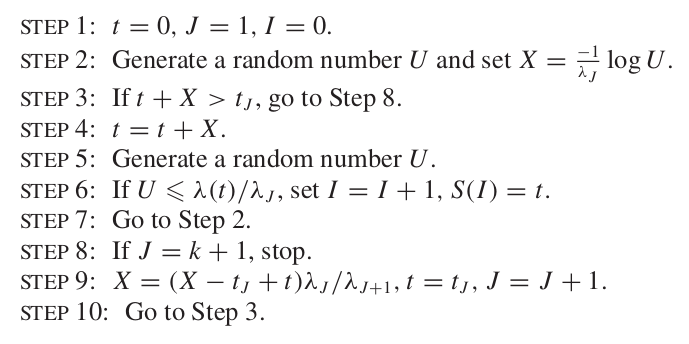
\includegraphics[width=0.6\textwidth]{0_images/nonHomogeneousAlgorithm.png}
    \caption{General non-homogeneous Poisson process simulation algorithm \cite{Ross2013GeneratingVariables}.}
    \label{fig:NonHomogeneousGeneralAlgorithm}
\end{figure}


\subsubsection{Stepwise Model Modified Simulation}
\label{sec:Method:PoissonSimulation:NonHomogeneousModified}
In the case of this project, the aforementioned intensity function $\lambda(t)$ is governed by the squared Euclidean distance between a given pair of nodes $(u,v)$, explained in section \ref{sec:Method:IntensityFunc}, and given by:

\begin{equation}
    \lambda_{u,v}(t)
    =
    \exp \left(\beta - ||\textbf{z}_u(t) - \textbf{z}_v(t)||_2^2\right)
    \label{eq:IntensityFunc2}
\end{equation}

First of all, this means that for each timestep ranging from $t_0$ to $t_0 + \Delta_{step}$, the non-homogeneous Poisson process has to be simulated for each of $\frac{N(N-1)}{2}$ node pairs.

Secondly, finding the upper bound $\lambda_U$ of a given intensity function $\lambda_{u,v}(t)$ is not straight forward, as the different intensity functions may be either be descending or ascending in the given step's time interval, and have a local minimum or maximum.
The explained method for simulating a non-homogeneous Poisson process using thinning is modified in order to accommodate for this difficulty.

For each node pair in each step, the monotonicity of the instensity function is found from looking at the sign around the roots of the derivative solved for zero of the intensity function.
For each step and node pair, the aforementioned $k$ time sub-intervals are now mapped along this found monotonicity, keeping track of the where the roots of the solved intensity function derivative are in relation to each sub-interval.
This means that a given sub-interval for time $[t_n,t_{n+1}]$ has the monotonicity corresponding to the sign of the derivative $\frac{d}{dt} \lambda_{u,v}(t)$ when between two roots.
If the sign is negative, ie. the monotonicity is decrasing, the upper bound intensity rate is set to $\lambda_U = \lambda_{u,v}(t)$.
If the monotonicity is increasing, the upper bound is set to $\lambda_U = \lambda_{u,v}(t+1)$.
In the cases the monotonicity changes from positive to negative for the next sub-interval, ie. passing a local maximum, the current sub-interval is positioned over a root, and gets the upper bound of $\lambda_U = \lambda_{u,v}(r)$.
If the monotonicity changes from negative to positive, the sub-interval is placed over a local minimum root, and must get the upper bound $\lambda_U = MAX(\lambda_{u,v}(t_n), \lambda_{u,v}(t_{n+1}))$
